\chapter{RESULTS DISCUSSION}
\label{chap-five}

\section*{Results Discussion}

This chapter will discuss the results presented in Chapter \ref{chap-four}.

\section{Material Consideration}

Various types of materials were used in the tests in the experiments.

\subsection{Commercial Material Categories}
The commercial tests were run on various samples. The samples were provided by Auralex Acoustics, and Eastman Chemical Company. There were 4 categories of materials tested. Various materials were tested within each of the $4$ categories. They were as follows:
\begin{enumerate}
	\item Sock Materials
		\begin{enumerate}
			\item Fiberglass Sock
			\item PET Sock
			\item Nylon Sock
		\end{enumerate}
	\item Raw Material Type
		\begin{enumerate}
			\item Raw Cotton Balls
			\item Auralex Compressed Cotton
		\end{enumerate}
	\item Acoustic Foam Type
		\begin{enumerate}
			\item Br�el \& Kj�r Foam
			\item Auralex Acoustics Foam
		\end{enumerate}
	\item Acoustic Panneling Type
		\begin{enumerate}
			\item Owens Corning Fiberglass Panel
			\item	Auralex Compressed Polyester Panel
		\end{enumerate}
\end{enumerate}
These categories represent each of the major types of absorption materials presently used today.

\subsection{Cellulose Acetate Material Categories}
The tests on the Cellulose Acetate can be broken down into 3 categories.
\begin{enumerate}
	\item Sock Materials
	\item Filter Rods
	\item Raw Tow
\end{enumerate}
These categories represent various types of manufacturing Cellulose Acetate in order to adequately analyze its utility as an absorption material.

\subsection{Matching Similar Commercial Materials to Cellulose Acetate}
To appropriately match the Cellulose Acetate material types to commercial materials, a wide range of materials were tested.\\
\indent The Sock materials provided much insight into Cellulose Acetates acoustic performance characteristics, and logically, were paired for comparison with the commercial sock materials. All of the Sock tests were performed using 4 and 8 layers of material to show a relationship between the thickness of absorption material present in the data.\\
\indent The Cellulose Acetate Filter Rods were compared against a few different materials, since there was not any directly similar material available. The rods were compared against raw cotton, and raw tow.\\
\indent The acoustic foams and paneling are commonly used commercially and were tested for data comparison.\\

\section{Considering Frequency Band}

In testing the materials two sizes of the impedance tubes were used. The large 100mm portion covered $50 \text{Hz}$ to $1600 \text{Hz}$ while the smaller 29mm portion covered $500 \text{Hz}$ to $6300 \text{Hz}$. It should be noted that for a theoretical impedance tube the working frequency range can span across a wide range of frequencies as noted in standards ISO-10534-2 \cite{ISO1998}, ASTM E1050-12 \cite{ASTM1990} and ASTM E2611-09 \cite{ASTM2011}. Calculations shown in Table \ref{tab:workingfreq} suggest that a larger frequency band may have been acceptable with this testing equipment. However the suggested frequencies by the tube's manufacturer were used.\\
\indent After collecting data on all samples which enough material was available for, it was determined that the smaller 29mm tube provided much better data than the larger tube which focused on lower frequencies. The broader range of data collected in the 29mm tube proved much more useful in showing the response of the materials. For this reason, a majority of the lower frequency data was thrown out. The presented data is that from the 29mm tube, e.g. $500 \text{Hz}$ to $6300 \text{Hz}$. Generally for human comfort level, the range between $2000 \text{Hz}$ and $4000 \text{Hz}$ is considered.

\section{Measurement Errors}
Each of these tests run in the Br�el \& Kj�r Impedance tube experienced small amounts of error due to imperfect materials and imperfect testing techniques. The performer of the experiment aimed to minimize these effects.

\subsection{Mechanical Resonance}
Mechanical resonance is caused when the skeletal structure of a porous material hits a frequency that matches the skeletal structure's natural frequency of vibration. Certain commercial and Cellulose materials present mechanical resonance which results in increased absorption within a narrow frequency range surrounding the natural frequency of vibration of the skeletal structure.

\subsubsection{Sock Materials}
Some of the materials showed abrupt peaks in their Absorption across the frequency spectrum. In particular, Figures \ref{fig:AuralexFoam}, \ref{fig:RawFiberglassThick}, \ref{fig:AfigSOCK8-2}, \ref{fig:AfigSOCK9-5}, \ref{fig:AfigSOCK9-6}, \ref{fig:AfigSOCK18-3}, \ref{fig:AfigSOCK18-4} showed a spike in absorption coefficient around $2000 \text{Hz}$. This is because these materials have a higher denier and thus were stiffer than the other samples. This resulted in the skeletal structure of the material hitting its resonant frequency. When the mode of the resonant frequency is excited, a small frequency band surrounding the center resonant frequency experience a higher amount of absorption.

\subsubsection{Filter Rod Materials}
The tests on the filter rod materials also presented some peaks in the lower frequency ranges due to the stiffer material hitting its resonance frequency. Figures \ref{fig:Afigfilterrodwhite}, and \ref{fig:Afigfilterrodblack} show a spike in the $1000 \text{Hz}$ to $2000 \text{Hz}$ range for samples with paper attached. The same samples tested without paper in figures \ref{fig:Afigfilterrodwhitenopaper}, and \ref{fig:Afigfilterrodblacknopaper} show a mechanical resonance spike in a similar range. This is more difficult to see due to the higher frequencies showing slightly different values.

\subsection{O-ring Considerations}
The testing set up on the Sock type materials needs to be considered. In order to allow the Sock materials to properly lay in the testing region, the samples were stapled to a rubber O-ring material. This O-ring provided some noise in the measurement. Tests were run in the Impedance Tube using only the O-ring. It can be seen in Figure \ref{fig:AfigOring} that the O-ring provided some additionally read absorption in the high frequencies. However, this can be ignored when it is compared with the measured reading in the empty tube in Figure \ref{fig:Afigempty}. 

\subsection{Air Gaps}
In an impedance tube measurement system, any present air gaps result in recording a higher value of absorption coefficient. This results in data that is not true to the materials absorption characteristics. This means that air gaps may have resulted in some data collected by the analysis system being inaccurate. This is an inevitability of an imperfect process of creating test samples as limited by the resources available.

\subsubsection{Filter Rod Materials}
The filter rod tests performed well as can be seen in the papered tests figures \ref{fig:Afigfilterrodwhite}, \ref{fig:Afigfilterrodblack} and the paperless tests figures \ref{fig:Afigfilterrodwhitenopaper} and \ref{fig:Afigfilterrodblacknopaper}. However, each of these tests had significant air gaps present. In order to properly input the filter rods into the impedance tube, the filter rods had to be packed in the diameter of the rubber O-ring for support. The air gaps are clearly seen in Figure \ref{fig:CircleInCircle}, which shows yellow filter rods, and the white air gaps.\\

\begin{figure}[hbtp]
    \centering
    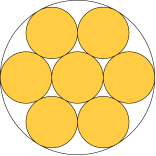
\includegraphics[width=0.3\textwidth]{Chapter-5/figs/CircleInCircle}
    \caption{Air Gap in Filter Rod Test - Yellow is Filter Rods, White is Air Gap }%\cite{Circle}}
    \label{fig:CircleInCircle}
\end{figure}

This percentage of air gap means that the filter rods data is artificially higher than the true value should be. In order to correct this error, filter rods of the exact size of the impedance tube (29mm) would need to be manufactured and tested to eliminate the air gap error. However, due to resources available, this test was unable to be performed.

\section{Health Impact}
A tremendous benefit to Cellulose Acetate Tow as an absorption material is its biocompatibility. Fibrous materials generally have their strongest absorption effects at higher frequencies, while lower frequencies have lower absorption effects. This is true for current industry standards. However, Cellulose Acetate provides similar performance characteristics to that of fiberglass. This allows Cellulose Acetate to be considered for use in environments when fiberglass would be unacceptable. An example of this would be an environment requiring no health risks, however, suffers from large durations and magnitudes of noise. An applicable environment could be medical in nature, such as a hospital emergency unit would require. The ability for designers to control the acoustic level in such an environment would be greatly benefit the patients and employees.

\section{Cost}
Results show Cellulose Acetate is a good alternative to commercial absorption materials. However, this must be looked at in regards to cost of the material. Fiberglass is a popular material in the absorption field. Part of the reason it is so popular is it is extremely cheap. Cellulose Acetate is more difficult to manufacture and consequently more expensive. However this premium comes with the added benefit of biofriendliness.\\
\indent Within the CA samples, there are some clear differences. The best overall performing was the Sock sample label 9-5 Figure \ref{fig:AfigSOCK9-5}, which had a Total Denier of 1576, a DPF of 2, 788 Filaments, and a Y cross section. However, this material is more difficult to work with than some of the relatively lower denier CA samples. The larger fiber size of the High Denier samples can be messy to work with. After working with one of these materials, lots of smaller particles get everywhere, which depending on the situation would not be ideal. This logistical cost is much higher than that of the lower denier finer knit fibers. These are easy to work with and do not get as messy as the larger ones. Pending on the situation, a higher denier or lower denier with many layer type of Tow would be needed.\\
\indent The CA sample labeled 9-3 Figure \ref{fig:AfigSOCK9-3}, which has a Total Denier of 150, a DPF of 6, 25 filaments, and a 8 Leg cross section, showed poor absorption performance, but has a better logistical cost. Since it has fine fibers, it is much easier to work with and depending on the scenario could be the ideal choice. The performance can be increased by using multiple layers.
